% !TEX root = ../../../main.tex

\toggletrue{image}
\toggletrue{imagehover}
\chapterimage{encoding_2x}
\chapterimagetitle{\uppercase{Encoding}}
\chapterimageurl{https://xkcd.com/1209/}
\chapterimagehover{I don't see how; the C0 block is right there at the beginning.}

\chapter{Was ist ein Code?}
\label{chapter-was-ist-ein-code}

In unserem Alltag treffen wir häufig auf Codes\footnote{Auch die Schreibweise Kode ist akzeptiert.}. Oft werden Zeichen oder Farben verwendet, die eine gewisse Bedeutung besitzen. Die Ampel (siehe \autoref{figure-ampel}) zeigt uns mit Farben an: Stop, Ready, Go. Bei Elektrogeräten wird mit Buchstaben der Energieverbrauch (siehe \autoref{figure-energie}) gekennzeichnet. Ein A bedeutet hier einen niedrigen Bedarf an Energie und ein G steht für einen hohen Bedarf an Energie. Und die Bedeutung der Zeichen aus \autoref{figure-abspielgeraet} sind seit den Kassettenrekordern bekannt: Aufnehmen, Abspielen, Pause und Stop.

\begin{figure}[htb]
\centering
\begin{minipage}{0.3\textwidth}
\centering
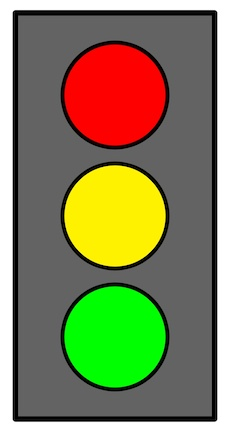
\includegraphics[scale=0.25]{ampel}
%https://www.publicdomainpictures.net/pictures/260000/velka/traffic-light-1526166819zss.jpg
\caption{Ampel.}
\label{figure-ampel}
\end{minipage}
\hfill
\begin{minipage}{0.3\textwidth}
\centering
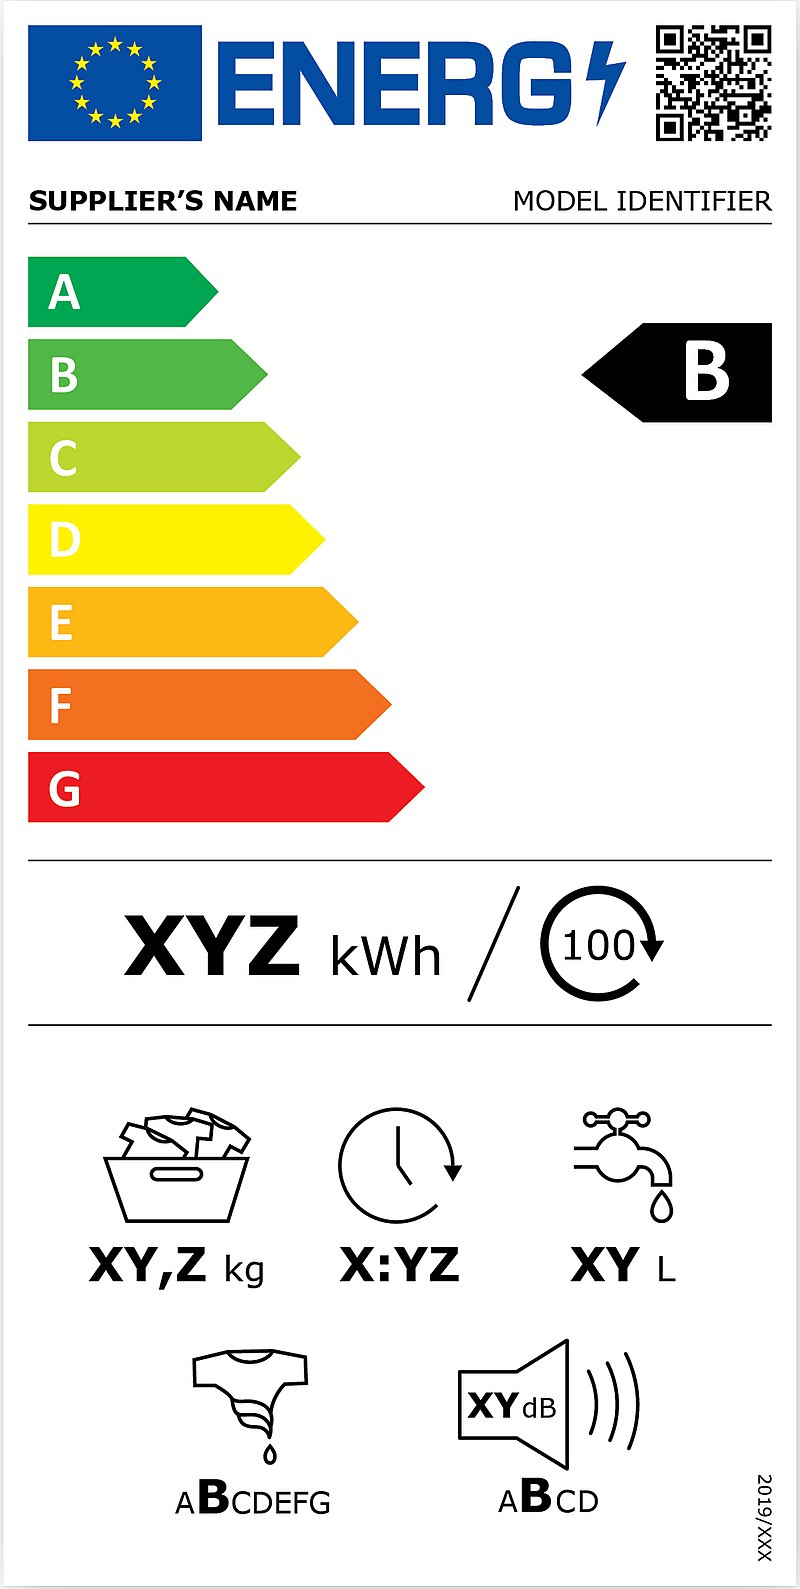
\includegraphics[scale=0.07]{eu_washing_machines_label}
%https://de.wikipedia.org/wiki/Energieverbrauchskennzeichnung#/media/Datei:EU_washing_machines_label.jpg
\caption{Energieverbrauchskennzeichnung.}
\label{figure-energie}
\end{minipage}
\hfill
\begin{minipage}{0.3\textwidth}
\centering
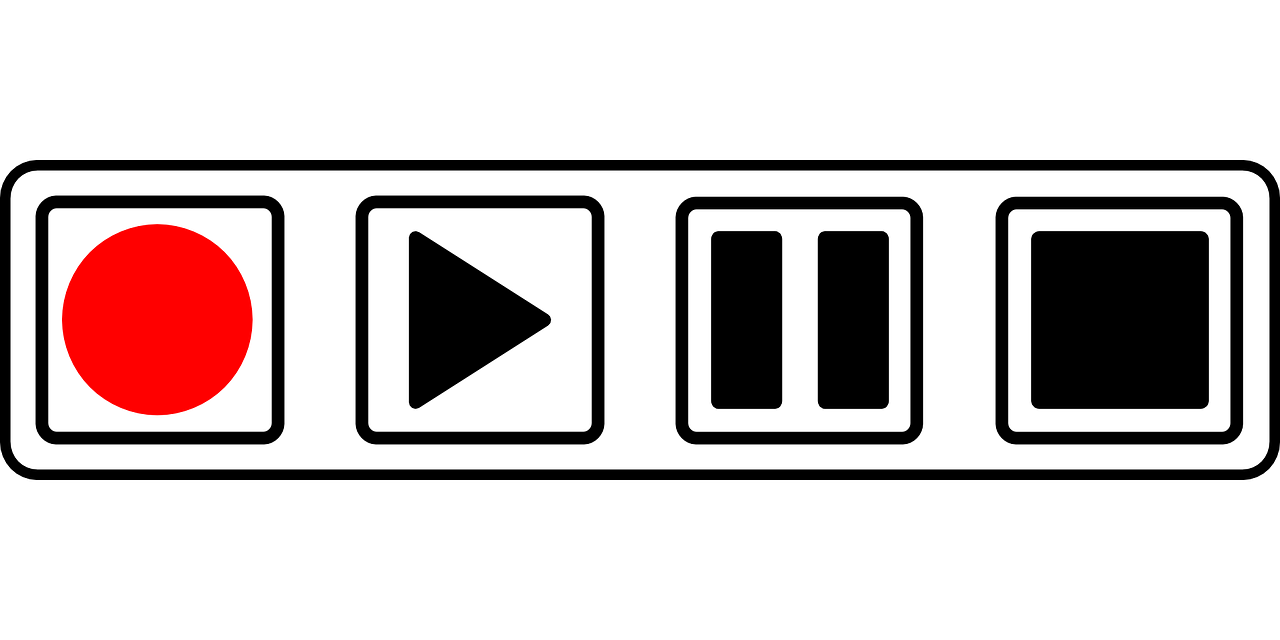
\includegraphics[scale=0.1]{start_stop_play}
%https://pixabay.com/de/vectors/tasten-anschlag-spielen-anhalten-35531/
\caption{Zeichen bei Abspielgeräten.}
\label{figure-abspielgeraet}
\end{minipage}
\end{figure}

\begin{figure}[htb]
\centering
\begin{minipage}{0.3\textwidth}
\centering
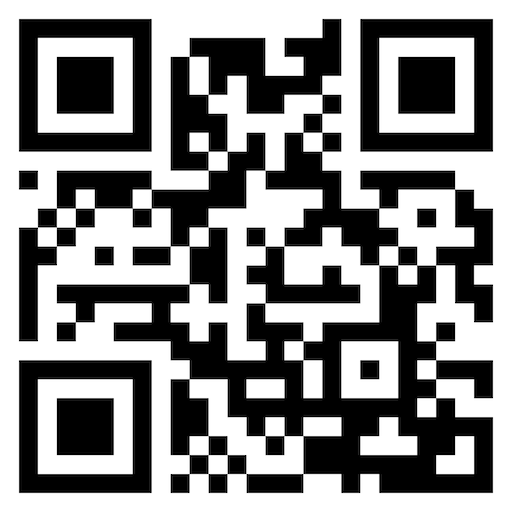
\includegraphics[scale=0.15]{qr_code}
%https://de.wikipedia.org/wiki/QR-Code#/media/Datei:QR_deWP.svg
\caption{Der Text \url{https://de.wikipedia.org} als \protect\acs{QR}-Code.}
\label{figure-qr-code}
\end{minipage}
\hfill
\begin{minipage}{0.3\textwidth}
\centering
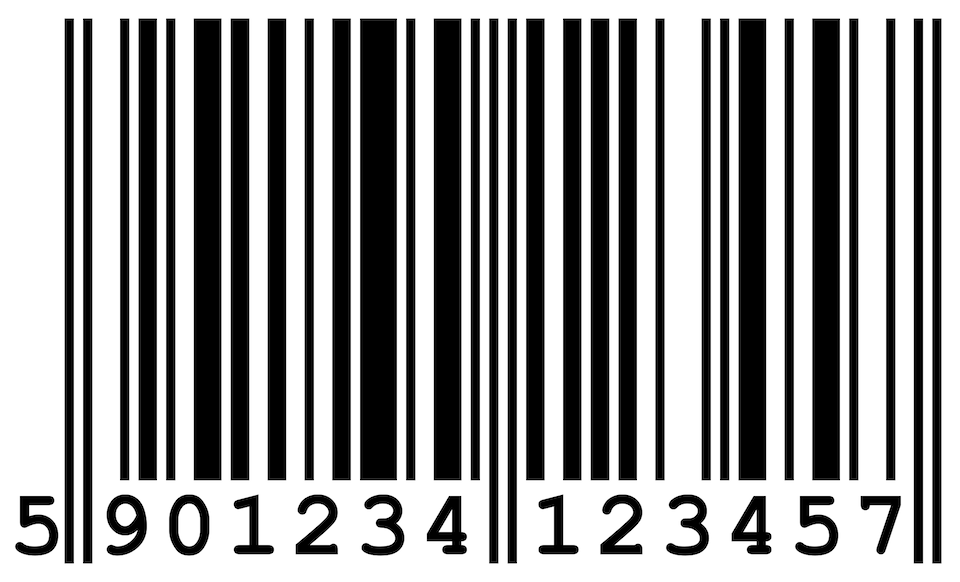
\includegraphics[scale=0.1]{ean13}
%https://de.wikipedia.org/wiki/Energieverbrauchskennzeichnung#/media/Datei:EU_washing_machines_label.jpg
\caption{\acs{EAN}-13 Strichcode.}
\label{figure-ean}
\end{minipage}
\hfill
\begin{minipage}{0.3\textwidth}
\centering
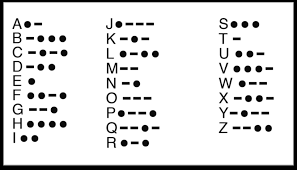
\includegraphics[scale=0.4]{morse}
%https://mia.phsz.ch/pub/Sekundarstufe/Codierung/2017-05-02-codes.pdf
\caption{Morsecode: Buchstaben werden zu Tönen}
\label{figure-morsealphabet}
\end{minipage}
\end{figure}

Auch in der Informatik spielen Codes eine wichtige Rolle. Ohne Codes könnten wir nicht programmieren. Keine Bilder speichern oder Nachrichten übertragen. Wir wollen uns in diesem Kapitel zunächst mit den wichtigsten Begriffen vertraut machen. Dann schauen wir uns als Beispiel den Morsecode an. Ab dem nächsten Kapitel beschäftigen wir uns dann mit Codes, welche der Computer benutzt. Die Lernziele lauten:

\newcommand{\codeLernziele}{
\protect\begin{todolist}
\item Sie definieren die Begriffe Code, Codierung und Decodierung.
\item Sie erklären die Begriffe am Beispiel des Morsecodes.
\item Sie erklären warum ein Code eindeutig decodierbar sein muss.
\item Sie erklären, was ein Binärcode ist.
\end{todolist}
}

\lernziel{\autoref{chapter-was-ist-ein-code}, \nameref{chapter-was-ist-ein-code}}{\protect\codeLernziele}

\codeLernziele

\section{Definitionen}

In der Informatik geht es bei Codes nicht um geheime Nachrichten. Es geht eigentlich meist darum, wie wir Daten in der für den Menschen verständlichen Form in eine für den Computer (oder ein anderes elektronisches Gerät) verarbeitbare Form umwandeln.

\begin{definition}[Code]
Ein Code ist eine Vorschrift, die beschreibt, wie wir Daten von einer Darstellung in eine andere Darstellung umwandeln. Dabei dürfen keine Daten verloren gehen. Eine eindeutige Rückumwandlung muss immer möglich sein. Die Vorschrift zur Umwandlung kann durch eine Code-Tabelle, eine mathematische Formel oder ein \say{Kochrezept} notiert werden.
\end{definition}

\begin{example}
\autoref{table-morse} zeigt einen Teil des \textbf{Morsecodes}. Beim Morsecode geht es darum, Zeichen durch kurze und lange Tonfolgen zu ersetzen. Diese Tonfolgen können dann mittels Funk übertragen werden. Amateurfunk, Luft- und Schifffahrt verwenden noch heute den Morsecode. 

\begin{table}[htb]
\centering
\begin{tabular}{|c|c||c|c||c|c|}
\hline
\textbf{Zeichen} & \textbf{Code-Wort} & \textbf{Zeichen} & \textbf{Code-Wort} & \textbf{Zeichen} & \textbf{Code-Wort} \\ \hline
A & $\cdot~-$ & J & $\cdot~-~-~-~$ & S & $\cdot~\cdot~\cdot$ \\ \hline
B & $-~\cdot~\cdot~\cdot$ & K & $-~\cdot~-$ & T & $-$ \\ \hline
C & $-~\cdot~-~\cdot$ & L & $\cdot~-\cdot~\cdot$ & U & $\cdot~\cdot~-$ \\ \hline
D &  $-~\cdot~\cdot$  & M & $-~-$ & V & $\cdot~\cdot~\cdot~-$ \\ \hline
E & $\cdot$ & N & $-~\cdot$ & W & $\cdot~-~-$ \\ \hline
F & $\cdot~\cdot~-~\cdot$ & O & $-~-~-~$ & X & $-~\cdot~\cdot~-$ \\ \hline
G & $-~-~\cdot$ & P & $\cdot~-~-~\cdot$  & Y & $-~\cdot~-~-$ \\ \hline
H & $\cdot~\cdot~\cdot~\cdot$ & Q & $-~-~\cdot~-$ & Z & $-~-~\cdot~\cdot~$ \\ \hline
I & $\cdot~\cdot$ & R & $\cdot~-~\cdot$ & @ & $\cdot~-~-~\cdot-~\cdot$ \\ \hline
\end{tabular}
\caption{Code-Tabelle für den Morsecode. Ein kurzer Ton ist durch einen Punkt dargestellt, ein langer Ton durch einen Strich.}
\label{table-morse}
\end{table}

\end{example}

Möchte man einen Code anwenden, so werden folgende Begriffe häufig eingesetzt.

\begin{definition}[Codieren und Decodieren]
Ein Code besteht aus Eingabedaten und Ausgabedaten. Das Umwandeln von Eingabedaten in Ausgabedaten nennt man Codieren (eng. encode). Beim Codieren entstehen Code-Wörter. Wandelt man ein Code-Wort zurück, dann spricht man von Decodieren (decode). 
\end{definition}

\begin{example}
Beim Morsecode sind die Eingabedaten die Zeichen A, B, C, D, $\dots$ und die Ausgabedaten die Tonfolgen. Wenn wir das Zeichen G codieren, dann erhalten wir $-~-~\cdot$. Decodieren wir das Code-Wort $-~\cdot~\cdot~-$, dann erhalten wir das Zeichen X.
\end{example}

\section{Eindeutig decodierbare Codes}

In unserem bisherigen Beispiel haben wir einzelnen Zeichen codiert. Nun kann man einen Code für einzelne Zeichen dazu verwenden, um ganze Wörter zu codieren.

\begin{example}
Wir codieren das Wort SOS mithilfe des Morsecodes. Beim Morsecode werden Wörter Zeichen für Zeichen codiert. Für das Wort SOS erhalten wir somit $\cdot~\cdot~\cdot~~-~-~-~~\cdot~\cdot~\cdot$.
\end{example}

Das Beispiel macht auf ein Problem aufmerksam. Betrachten wir die Zeichen $\cdot\cdot\cdot$ dann ist ein eindeutige \textbf{Decodierung} nicht möglich. Wir können es zum Beispiel als das Zeichen S decodieren oder drei Mal das Zeichen E. Es entstehen mehrere Möglichkeiten. Ein gültiger Code muss jedoch eine \textbf{eindeutige} Rückumwandlung ermöglichen. Somit ist der Code nicht gültig. Damit wir die Code-Wörter des Morse-Codes unterscheiden können, benötigen wir ein weiteres Zeichen. Zwischen zwei Code-Wörtern benötigt es ein \say{Trennelement} - die Pause ($/$). Für das Wort SOS erhalten wir somit $\cdot~\cdot~\cdot~/~-~-~-~/~\cdot~\cdot~\cdot$.

\begin{definition}[Eindeutig decodierbarer Code]
Ein Code heisst eindeutig decodierbar genau dann, wenn jedes Code-Wort nur auf eine einzige Art zurückübersetzt (decodiert) werden kann. Auch eine Folge von Code-Wörtern muss eindeutig decodierbar sein.
\end{definition}

Es müssen dabei nur Code-Wörter eindeutig decodierbar sein, welche zuvor korrekt codiert wurden. Nicht jedes beliebige Wort muss somit (eindeutig) decodierbar sein.

\section{Aufgaben}

\begin{enumerate}
\item Decodieren Sie $\cdot~\cdot~/-~\cdot~/~\cdot~\cdot~-~\cdot~/~-~-~-~/~\cdot~-~\cdot~/~-~-~/~\cdot~-~/~-~/~\cdot~\cdot~/~-~\cdot~-$.
\fillwithgrid{0.25in}
\item Codieren Sie Ihren Vornamen mit dem Morsecode. Verwenden Sie nur Grossbuchstaben.
\fillwithgrid{1in}
\item Zeigen Sie, dass $-~\cdot~-~\cdot~\cdot~\cdot~\cdot~-~-~\cdot$ nicht eindeutig decodiert werden kann (das Trennelement also wirklich notwendig ist).
\fillwithgrid{1in}
\end{enumerate}

\section{Binärcodes}

Ein Computer arbeitet mit Binärdaten. Aus diesem Grund sind wir vor allem an Codes interessiert, welche als Ausgabedaten nur Bits verwenden.

\begin{definition}[Binärcode]
Falls ein Code nur Code-Wörter mit den Zeichen $0$ und $1$ verwendet, dann handelt es sich um einen Binärcode.
\end{definition}

Wir fokussieren uns deshalb von nun an auf Binärcodes.

\begin{example}
Der Unicode ist ein Binärcode. Wir codieren den Text \say{Dies ist ein Binärcode.} mit dem Unicode in die folgenden Bits:

\begin{lstlisting}[language=output, caption={Leerzeichen und neue Zeilen dienen nur der Übersicht.}]
01000100 01101001 01100101 01110011 00100000 01101001
01110011 01110100 00100000 01100101 01101001 01101110
00100000 01000010 01101001 01101110 11000011 10100100
01110010 01100011 01101111 01100100 01100101 00101110
\end{lstlisting}

\end{example}